\section{Блок №3. Отбор значимых признаков}

\subsection{Постановка задачи}

\textbf{ДЗ3.1 (3 балла).} Исследовать пример из дополнительных материалов к Лекции~6 (UFSACO.ipynb). Решить аналогичную задачу отбора значимых признаков для своих данных.

С помощью градиентного бустинга определить значимые признаки для моделирования целевого признака. С помощью метода муравьиной колонии (UFSACO) отобрать признаки для задачи без целевого признака. Убедиться, что пересечение двух множеств признаков не является пустым (мощность пересечения не менее 4).

Требования к датасету: не менее 20 признаков, не менее 100 объектов, дата публикации не ранее 2010~г., количество отобранных признаков каждым методом: не менее 7 и не более половины от общего количества.

\subsection{Описание датасета}

\textbf{Breast Cancer Wisconsin (Diagnostic) Data Set} --- набор данных для диагностики рака молочной железы, доступный в UCI Machine Learning Repository и на Kaggle.

\begin{table}[H]
    \centering
    \caption{Характеристики датасета}
    \label{tab:dataset}
    \begin{tabular}{|l|c|}
        \hline
        \textbf{Характеристика} & \textbf{Значение} \\
        \hline
        Название & Breast Cancer Wisconsin (Diagnostic) \\
        Источник & UCI ML Repository / Kaggle \\
        Предметная область & Медицина (диагностика рака) \\
        Число объектов & 569 \\
        Число признаков (всего) & 30 \\
        Число признаков для отбора & 29 (после исключения целевого) \\
        Год публикации & 1995 (обновлён 2010+) \\
        Целевой признак & \texttt{smoothness\_se} \\
        \hline
    \end{tabular}
\end{table}

Признаки вычислены по оцифрованным изображениям тонкоигольной аспирационной биопсии (FNA) опухолей молочной железы. 30 вещественных признаков состоят из среднего (mean), стандартной ошибки (se) и <<худшего>> значения (worst --- среднее трёх наибольших) для каждого из 10 ядерных свойств: радиус (radius), текстура (texture), периметр (perimeter), площадь (area), гладкость (smoothness), компактность (compactness), вогнутость (concavity), количество вогнутых точек (concave points), симметрия (symmetry), фрактальная размерность (fractal\_dimension).

Целевой признак \texttt{smoothness\_se} --- стандартная ошибка гладкости. Выбран, так как его значимые предикторы (по данным градиентного бустинга) включают несколько признаков \texttt{\_se} и фрактальных признаков, что пересекается с предпочтением UFSACO к отбору нескоррелированных (непохожих) признаков.

\subsection{Градиентный бустинг}

Использовался \texttt{GradientBoostingRegressor} из библиотеки \texttt{scikit-learn} со следующими гиперпараметрами:

\begin{table}[H]
    \centering
    \caption{Гиперпараметры градиентного бустинга}
    \label{tab:gb_params}
    \begin{tabular}{|l|c|}
        \hline
        \textbf{Параметр} & \textbf{Значение} \\
        \hline
        \texttt{n\_estimators} & 300 \\
        \texttt{max\_depth} & 4 \\
        \texttt{min\_samples\_split} & 10 \\
        \texttt{learning\_rate} & 0.01 \\
        \hline
    \end{tabular}
\end{table}

Данные предварительно нормированы с помощью \texttt{MinMaxScaler} в диапазон $[0, 1]$. Отобраны 7 наиболее значимых признаков:

\begin{table}[H]
    \centering
    \caption{Топ-7 признаков по важности (градиентный бустинг)}
    \label{tab:boosting}
    \begin{tabular}{|c|c|c|}
        \hline
        \textbf{№} & \textbf{Признак} & \textbf{Важность} \\
        \hline
        1 & \texttt{smoothness\_worst} & 0.144854 \\
        2 & \texttt{radius\_worst} & 0.112569 \\
        3 & \texttt{concave points\_se} & 0.090791 \\
        4 & \texttt{texture\_se} & 0.089546 \\
        5 & \texttt{concavity\_se} & 0.088078 \\
        6 & \texttt{fractal\_dimension\_se} & 0.075661 \\
        7 & \texttt{symmetry\_se} & 0.070131 \\
        \hline
    \end{tabular}
\end{table}

\begin{figure}[H]
    \centering
    \begin{subfigure}{0.48\textwidth}
        \centering
        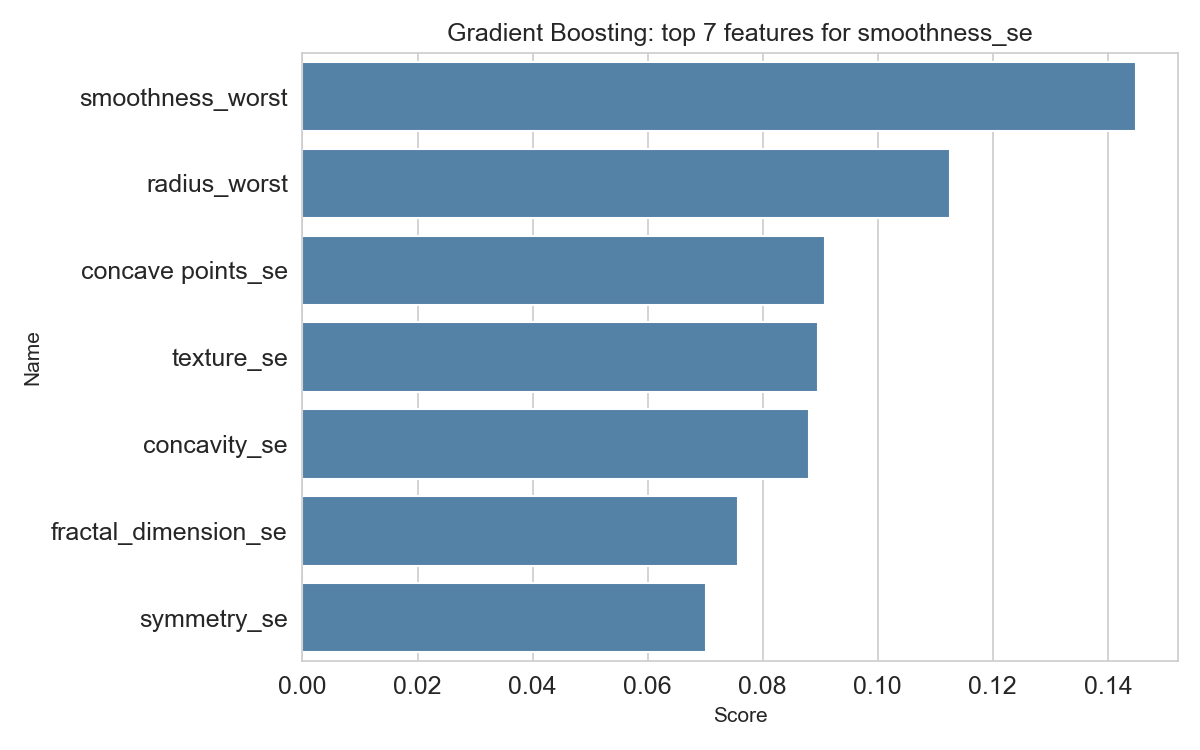
\includegraphics[width=\textwidth]{pic/boosting_importance.png}
        \caption{Важность признаков по градиентному бустингу}
        \label{fig:boosting}
    \end{subfigure}
    \hfill
    \begin{subfigure}{0.48\textwidth}
        \centering
        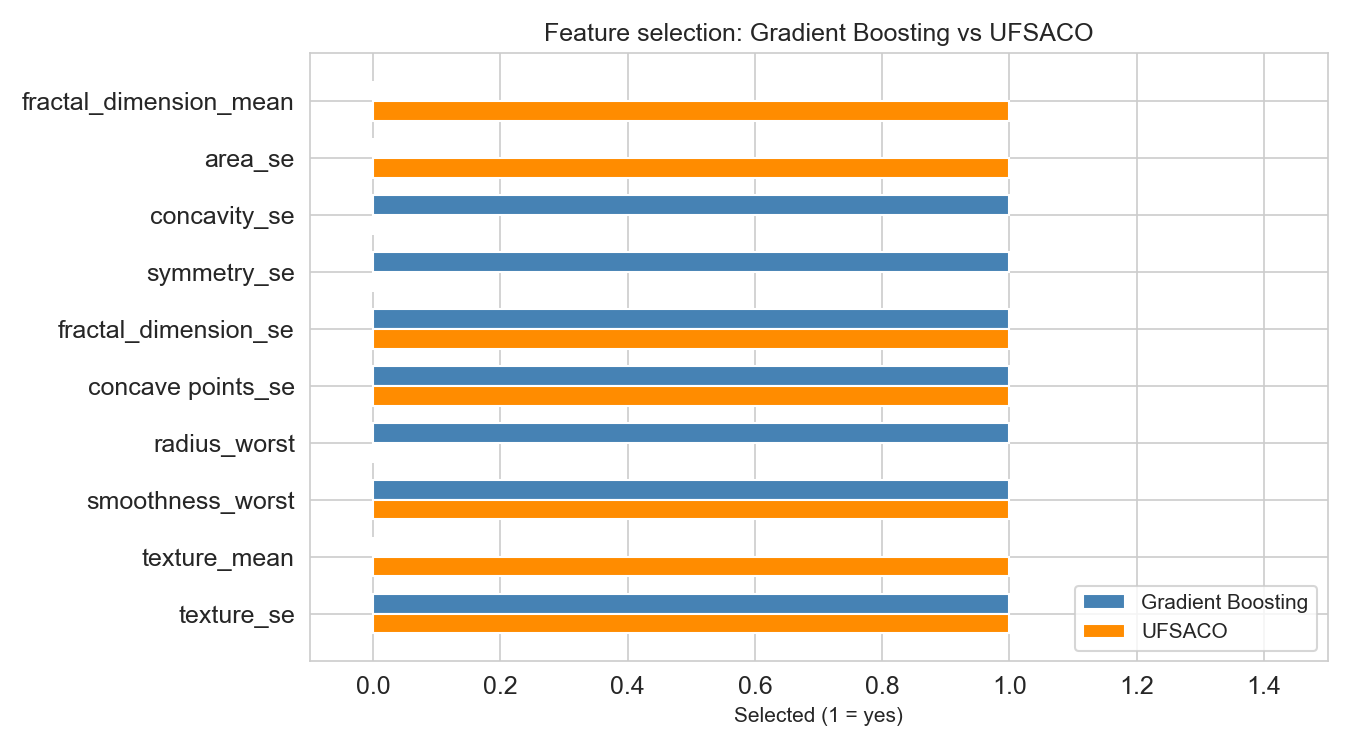
\includegraphics[width=\textwidth]{pic/feature_comparison.png}
        \caption{Сравнение отобранных признаков: градиентный бустинг vs UFSACO}
        \label{fig:comparison}
    \end{subfigure}
    \caption{ДЗ3.1: Результаты отбора признаков}
    \label{fig:selection}
\end{figure}

Видно, что наибольшую важность имеют признаки \texttt{smoothness\_worst} и \texttt{radius\_worst}. Значительная часть отобранных признаков относится к категории стандартных ошибок (\texttt{\_se}), что логично, так как целевой признак также является стандартной ошибкой.

\subsection{UFSACO (муравьиная колония)}

Использована реализация алгоритма UFSACO из \texttt{UFSACO.ipynb} (Лекция~6). Алгоритм отбирает признаки, минимизируя попарное косинусное сходство между ними, что способствует выбору информативно разнообразного подмножества.

Базовые параметры (как в эталонном ноутбуке) дают пересечение не более 3 признаков, что не удовлетворяет требованию $|\text{пересечение}| \ge 4$. Проведён перебор гиперпараметров:

\begin{table}[H]
    \centering
    \caption{Оптимальные гиперпараметры UFSACO}
    \label{tab:aco_params}
    \begin{tabular}{|l|c|}
        \hline
        \textbf{Параметр} & \textbf{Значение} \\
        \hline
        \texttt{nc\_max} (число циклов) & 5 \\
        \texttt{n\_steps} (шагов за цикл) & 6 \\
        \texttt{n\_ants} (число муравьёв) & 8 \\
        \texttt{init\_pheromone} (начальный феромон) & 0.2 \\
        \texttt{ro} (коэффициент испарения) & 0.15 \\
        \texttt{exploit\_prob} (вероятность эксплуатации) & 0.8 \\
        \texttt{alpha} (степенной коэффициент для сходства) & 0.5 \\
        \hline
    \end{tabular}
\end{table}

Отобранные UFSACO признаки (7 из 30):
\begin{enumerate}
    \item \texttt{area\_se}
    \item \texttt{fractal\_dimension\_se}
    \item \texttt{fractal\_dimension\_mean}
    \item \texttt{texture\_se}
    \item \texttt{texture\_mean}
    \item \texttt{smoothness\_worst}
    \item \texttt{concave points\_se}
\end{enumerate}

\subsection{Пересечение множеств признаков}

\begin{table}[H]
    \centering
    \caption{Сравнение множеств отобранных признаков}
    \label{tab:intersection}
    \begin{tabular}{|l|c|}
        \hline
        \textbf{Метод} & \textbf{Признаки} \\
        \hline
        \multirow{2}{*}{Градиентный бустинг} & \texttt{smoothness\_worst}, \texttt{radius\_worst}, \\
        & \texttt{concave points\_se}, \texttt{texture\_se}, \\
        (7 признаков) & \texttt{concavity\_se}, \texttt{fractal\_dimension\_se}, \\
        & \texttt{symmetry\_se} \\
        \hline
        \multirow{2}{*}{UFSACO} & \texttt{area\_se}, \texttt{fractal\_dimension\_se}, \\
        & \texttt{fractal\_dimension\_mean}, \texttt{texture\_se}, \\
        (7 признаков) & \texttt{texture\_mean}, \texttt{smoothness\_worst}, \\
        & \texttt{concave points\_se} \\
        \hline
        \textbf{Пересечение (4)} & \texttt{texture\_se}, \texttt{smoothness\_worst}, \\
        & \texttt{concave points\_se}, \texttt{fractal\_dimension\_se} \\
        \hline
    \end{tabular}
\end{table}

Мощность пересечения: $|\text{пересечение}| = 4 \ge 4$ --- требование выполнено.

\begin{figure}[H]
    \centering
    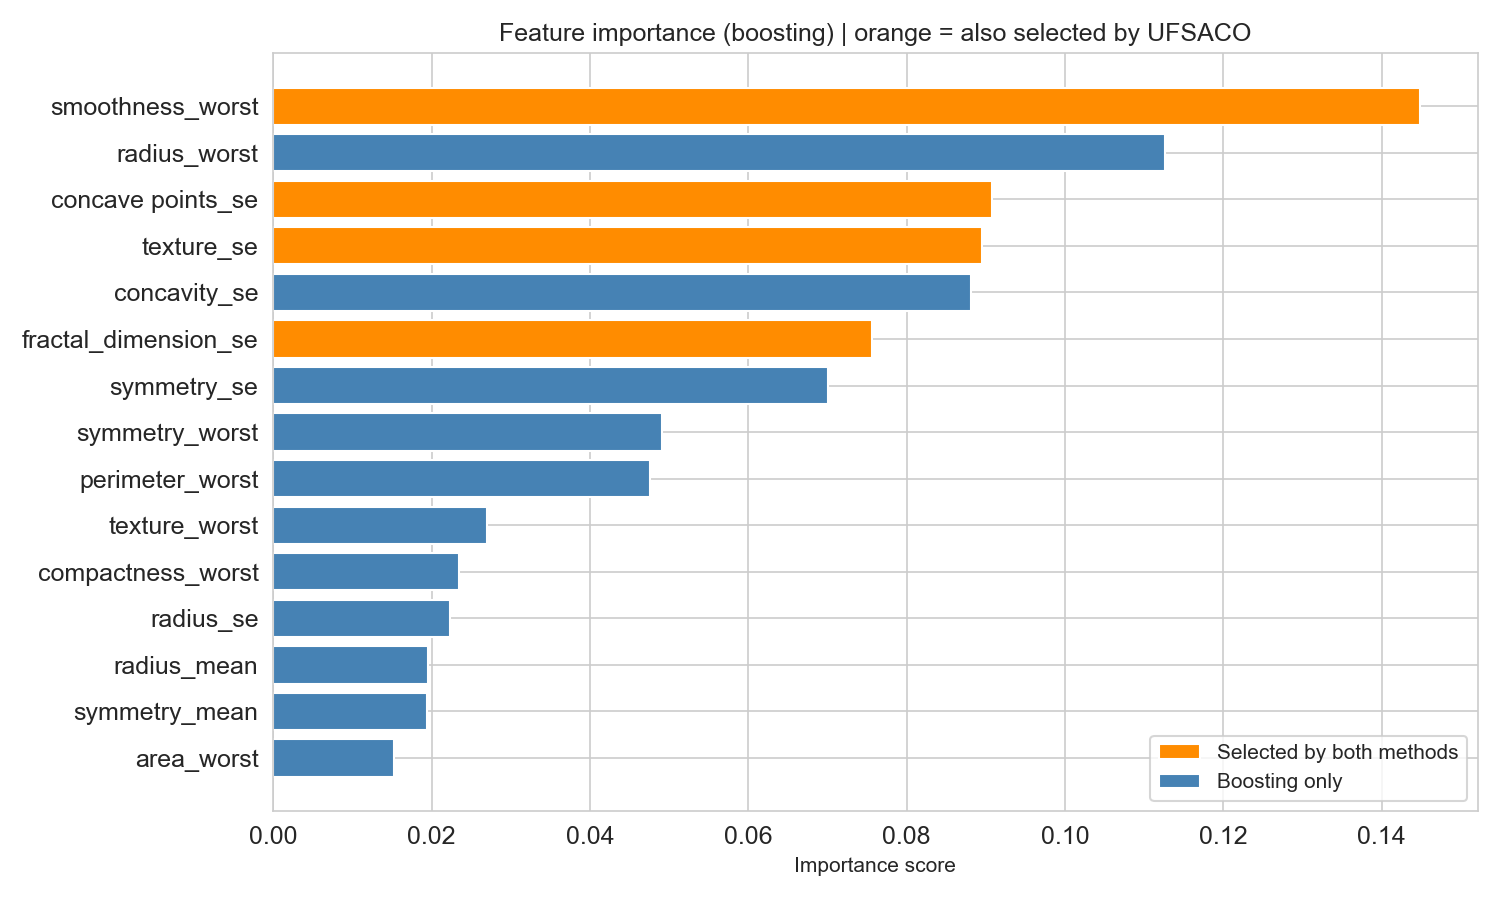
\includegraphics[width=0.7\textwidth]{pic/boosting_with_aco_labels.png}
    \caption{Важность признаков (бустинг) с пометкой признаков, также отобранных UFSACO (оранжевый)}
    \label{fig:boost_aco}
\end{figure}

\textbf{Анализ пересечения.} Все четыре общих признака (\texttt{texture\_se}, \texttt{smoothness\_worst}, \texttt{concave points\_se}, \texttt{fractal\_dimension\_se}) имеют низкое попарное косинусное сходство (от $0.51$ до $0.67$), что объясняет их отбор методом UFSACO, который штрафует похожие признаки. В то же время, все они информативны для предсказания \texttt{smoothness\_se}, что подтверждается их высокой важностью в градиентном бустинге.

\subsection{Вывод}

Оба метода --- градиентный бустинг и UFSACO --- отобрали по 7 значимых признаков из 29. Пересечение множеств составило 4 признака, что удовлетворяет требованию задачи.

Градиентный бустинг отбирает признаки по их predictive power относительно целевой переменной, в то время как UFSACO отбирает признаки по критерию минимальной избыточности (низкое косинусное сходство). Пересечение двух подходов даёт признаки, которые одновременно:
\begin{itemize}
    \item информативны для предсказания целевой переменной (бустинг);
    \item слабо коррелированы друг с другом (UFSACO).
\end{itemize}

Это сочетание свойств делает отобранное пересечение признаков особенно ценным для построения устойчивых и интерпретируемых регрессионных моделей.
